% =====================================================================
% File        : operasi_matriks_matlab.tex
% Deskripsi   : Operasi matriks di MATLAB: +, -, perkalian, transpose, det, inv, eigen
%               dengan contoh A = magic(4)
% =====================================================================
\documentclass[aspectratio=169,11pt]{beamer}
\usetheme{metropolis}
\usepackage[utf8]{inputenc}
\usepackage{amsmath,amssymb}
\usepackage{booktabs}
\usepackage{listings}
\usepackage{tikz}
\usetikzlibrary{matrix,positioning,arrows.meta,fit,calc}

% Matriks A = magic(4) dengan label indeks baris/kolom; #1 = anotasi tambahan
\newcommand{\Amat}[1]{%
\begin{tikzpicture}
\matrix (m) [matrix of math nodes, ampersand replacement=\&,
             nodes={minimum width=2.8em, minimum height=1.7em},
             left delimiter={[}, right delimiter={]}]
{ 16 \& 2 \& 3 \& 13\\
  5 \& 11 \& 10 \& 8\\
  9 \& 7 \& 6 \& 12\\
  4 \& 14 \& 15 \& 1\\ };
\foreach \c in {1,...,4}
  \node[font=\scriptsize, text=gray] at ([yshift=8pt]m-1-\c.north) {\c};
\foreach \r in {1,...,4}
  \node[font=\scriptsize, text=gray] at ([xshift=-16pt]m-\r-1.west) {\r};
#1
\end{tikzpicture}}

\definecolor{kolom}{RGB}{31,119,180}
\definecolor{baris}{RGB}{214,39,40}
\definecolor{kode}{RGB}{245,245,245}
\newcommand{\z}{\textcolor{gray!45}{0}}

\lstset{
  language=Matlab,
  basicstyle=\ttfamily\small,
  backgroundcolor=\color{kode},
  keywordstyle=\color{kolom}\bfseries,
  commentstyle=\color{gray}\itshape,
  frame=single, rulecolor=\color{gray!40},
  columns=fullflexible, keepspaces=true,
  xleftmargin=4pt, xrightmargin=4pt
}

\title{Operasi Matriks di MATLAB}
\subtitle{Penjumlahan, perkalian, transpose, determinan, invers, dan eigen}
\author{Andreas Syaloom Kurniawan}
\institute{Faculty of Economics and Business, Universitas Gadjah Mada}
\date{}

\begin{document}

\maketitle

% ---------------------------------------------------------------------
\begin{frame}[fragile]{Matriks yang dipakai di slide ini}
\begin{columns}[T]
\column{0.5\textwidth}
\small
\[
P=\begin{bmatrix}1&2\\3&4\end{bmatrix},\quad
Q=\begin{bmatrix}5&6\\7&8\end{bmatrix}
\]
\[
C=\begin{bmatrix}1&2&3\\4&5&6\end{bmatrix},\quad
S=\begin{bmatrix}2&1\\1&2\end{bmatrix}
\]
\[
A=\texttt{magic(4)}=
\begin{bmatrix}
16&2&3&13\\5&11&10&8\\9&7&6&12\\4&14&15&1
\end{bmatrix}
\]
\column{0.46\textwidth}
\begin{lstlisting}[basicstyle=\ttfamily\footnotesize]
P = [1 2; 3 4];
Q = [5 6; 7 8];
C = [1 2 3; 4 5 6];
S = [2 1; 1 2];
A = magic(4);
\end{lstlisting}
\small Jalankan blok ini dulu agar semua contoh dapat diikuti.
\end{columns}
\end{frame}


\begin{frame}[fragile]{Penjumlahan dan pengurangan}
\[
P=\begin{bmatrix}1&2\\3&4\end{bmatrix},\quad
Q=\begin{bmatrix}5&6\\7&8\end{bmatrix}
\qquad
P+Q=\begin{bmatrix}6&8\\10&12\end{bmatrix},\quad
P-Q=\begin{bmatrix}-4&-4\\-4&-4\end{bmatrix}
\]
\begin{columns}[T]
\column{0.48\textwidth}
\begin{lstlisting}[basicstyle=\ttfamily\footnotesize]
>> P = [1 2; 3 4];
>> Q = [5 6; 7 8];
>> P + Q
>> P - Q
>> P + 10     % tambah skalar
\end{lstlisting}
\column{0.48\textwidth}
\small
\begin{itemize}
  \item Elemen demi elemen: $(P\pm Q)_{ij} = p_{ij}\pm q_{ij}$.
  \item Syarat: \alert{ukuran sama} (atau kompatibel lewat
        \emph{implicit expansion}, R2016b+).
  \item \texttt{magic(4) + eye(3)} $\rightarrow$ error ukuran.
\end{itemize}
\end{columns}
\end{frame}

% ---------------------------------------------------------------------
\begin{frame}[fragile]{Perkalian matriks: \texttt{A*B}}
\begin{columns}[T]
\column{0.52\textwidth}
\small
Syarat: \alert{kolom $A$ = baris $B$}.
\[
(m\times\textcolor{baris}{n})\,(\textcolor{baris}{n}\times p) \;\rightarrow\; m\times p,
\qquad
c_{ij} = \sum_{k=1}^{n} a_{ik}\,b_{kj}
\]
Baris $i$ dari $P$ ``dikali-jumlahkan'' dengan kolom $j$ dari $Q$:
\[
PQ=\begin{bmatrix}
1\cdot5+2\cdot7 & 1\cdot6+2\cdot8\\
3\cdot5+4\cdot7 & 3\cdot6+4\cdot8
\end{bmatrix}
=\begin{bmatrix}19&22\\43&50\end{bmatrix}
\]
\column{0.44\textwidth}
\begin{lstlisting}[basicstyle=\ttfamily\scriptsize]
>> P * Q
ans =
    19    22
    43    50
>> Q * P
ans =
    23    34
    31    46
>> C = [1 2 3; 4 5 6];
>> C * C'      % (2x3)(3x2)
>> C * C       % error (slide berikut)
\end{lstlisting}
\small Umumnya $PQ \neq QP$ (\alert{tidak komutatif}).
\end{columns}
\end{frame}

% ---------------------------------------------------------------------
\begin{frame}[fragile]{Jika dimensi tidak cocok pada \texttt{A*B}}
\begin{lstlisting}[basicstyle=\ttfamily\scriptsize, deletekeywords={for}]
>> C * C        % (2x3)(2x3): kolom C = 3, baris C = 2
Error using  *
Incorrect dimensions for matrix multiplication. Check that the number of
columns in the first matrix matches the number of rows in the second matrix.
To operate on each element of the matrix individually, use TIMES (.*) for
elementwise multiplication.
\end{lstlisting}
\scriptsize MATLAB versi lama: \texttt{Inner matrix dimensions must agree.}

\vspace{0.4em}
\begin{columns}[T]
\column{0.48\textwidth}
\small
\begin{itemize}
  \item \textbf{Skalar selalu lolos}: \texttt{3*C} dan \texttt{C*3} tidak pernah error.
  \item \textbf{Solusi biasanya transpose}, bukan \texttt{.*}:
        \texttt{C*C'} ($2\times2$) atau \texttt{C'*C} ($3\times3$).
\end{itemize}
\column{0.48\textwidth}
\small
\textcolor{baris}{\textbf{Jebakan \texttt{.*}}}: sejak R2016b ada
\emph{implicit expansion}.
\begin{lstlisting}[basicstyle=\ttfamily\scriptsize]
>> a = [1;2;3];  b = [4 5 6];
>> a .* b      % TIDAK error -> 3x3
>> C .* C'     % (2x3).*(3x2) -> error:
Arrays have incompatible sizes ...
\end{lstlisting}
\end{columns}
\end{frame}

% ---------------------------------------------------------------------
\begin{frame}[fragile]{Perkalian skalar: \texttt{k*A}}
\begin{columns}[T]
\column{0.5\textwidth}
\small
Setiap elemen dikalikan bilangan $k$:
\[
(kA)_{ij} = k\,a_{ij}
\]
\[
3P = 3\begin{bmatrix}1&2\\3&4\end{bmatrix}
= \begin{bmatrix}3&6\\9&12\end{bmatrix}
\]
Sifat:
\begin{itemize}
  \item $kA = Ak$ (urutan bebas)
  \item $k(A+B) = kA + kB$
  \item $\det(kA) = k^n \det(A)$ untuk $A$ $n\times n$
\end{itemize}
\column{0.46\textwidth}
\begin{lstlisting}[basicstyle=\ttfamily\footnotesize]
>> 3 * P
ans =
     3     6
     9    12
>> P * 3       % sama
>> P / 2       % = 0.5 * P
>> det(3*P)    % 9 * det(P) = -18
\end{lstlisting}
\small Untuk skalar, \texttt{*} dan \texttt{.*} memberi hasil yang sama.
\end{columns}
\end{frame}

% ---------------------------------------------------------------------
\begin{frame}[fragile]{Perkalian Kronecker: \texttt{kron(A,B)}}
\begin{columns}[T]
\column{0.54\textwidth}
\small
Setiap elemen $a_{ij}$ diganti dengan \alert{blok} $a_{ij}B$:
\[
P\otimes Q =
\begin{bmatrix}
1\cdot Q & 2\cdot Q\\
3\cdot Q & 4\cdot Q
\end{bmatrix}
=
\left[\begin{array}{cc|cc}
5&6&10&12\\
7&8&14&16\\ \hline
15&18&20&24\\
21&24&28&32
\end{array}\right]
\]
Ukuran: $(m\times n)\otimes(p\times q) \rightarrow mp\times nq$.
Tidak ada syarat ukuran.
\column{0.42\textwidth}
\begin{lstlisting}[basicstyle=\ttfamily\footnotesize]
>> kron(P, Q)       % 4x4
>> size(kron(C, P))
ans =
     4     6
>> kron(eye(2), P)  % blok diag
ans =
     1     2     0     0
     3     4     0     0
     0     0     1     2
     0     0     3     4
\end{lstlisting}
\scriptsize Contoh pemakaian: matriks kovarians SUR/VAR, $\Sigma\otimes I_T$.
\end{columns}
\end{frame}

% ---------------------------------------------------------------------
\begin{frame}[fragile]{Transpose: \texttt{A'} dan \texttt{A.'}}
\begin{columns}[c]
\column{0.48\textwidth}
\centering
\[
C=\begin{bmatrix}1&2&3\\4&5&6\end{bmatrix}
\;\Rightarrow\;
C'=\begin{bmatrix}1&4\\2&5\\3&6\end{bmatrix}
\]
\small Baris menjadi kolom: $(C')_{ij} = c_{ji}$,\\
ukuran $2\times3 \rightarrow 3\times2$.
\column{0.48\textwidth}
\begin{lstlisting}[basicstyle=\ttfamily\footnotesize]
>> C = [1 2 3; 4 5 6];
>> C'        % transpose konjugat
>> C.'       % transpose biasa
>> isequal(A', A)
ans = 0      % magic(4) tidak simetris
\end{lstlisting}
\small Untuk bilangan real, \texttt{'} dan \texttt{.'} sama. Untuk kompleks,
\texttt{'} juga mengonjugasi.
\end{columns}
\end{frame}

% ---------------------------------------------------------------------
\begin{frame}[fragile]{Determinan: \texttt{det}}
\begin{columns}[T]
\column{0.5\textwidth}
\small
Untuk matriks $2\times2$:
\[
\det\begin{bmatrix}a&b\\c&d\end{bmatrix} = ad-bc
\]
\[
\det(P) = 1\cdot4 - 2\cdot3 = -2
\]
Makna geometris: $|\det|$ = faktor perubahan \alert{luas} (atau volume)
oleh transformasi; tanda negatif berarti orientasi terbalik.
\column{0.46\textwidth}
\begin{lstlisting}[basicstyle=\ttfamily\footnotesize]
>> det(P)
ans = -2.0000
>> det(magic(4))
ans = -1.4495e-12
>> rank(magic(4))
ans = 3
\end{lstlisting}
\small \texttt{magic(4)} singular: determinan seharusnya $0$, tetapi
pembulatan floating point memberi angka sangat kecil. Cek singularitas
dengan \texttt{rank} atau \texttt{cond}, bukan \texttt{det}.
\end{columns}
\end{frame}

% ---------------------------------------------------------------------
\begin{frame}[fragile]{Invers: \texttt{inv} dan operator \texttt{\textbackslash}}
\begin{columns}[T]
\column{0.5\textwidth}
\small
Untuk $2\times2$ dengan $\det\ne0$:
\[
\begin{bmatrix}a&b\\c&d\end{bmatrix}^{-1}
= \frac{1}{ad-bc}\begin{bmatrix}d&-b\\-c&a\end{bmatrix}
\]
\[
P^{-1} = \frac{1}{-2}\begin{bmatrix}4&-2\\-3&1\end{bmatrix}
= \begin{bmatrix}-2&1\\1.5&-0.5\end{bmatrix}
\]
Sifat: $PP^{-1} = P^{-1}P = I$.
\column{0.46\textwidth}
\begin{lstlisting}[basicstyle=\ttfamily\footnotesize]
>> inv(P)
ans =
   -2.0000    1.0000
    1.5000   -0.5000
>> P * inv(P)       % = eye(2)
>> inv(magic(4))    % warning: singular
\end{lstlisting}
\small Untuk menyelesaikan $Px=b$, gunakan \texttt{x = P\textbackslash b}
(lebih cepat dan stabil) daripada \texttt{inv(P)*b}.
\end{columns}
\end{frame}

% ---------------------------------------------------------------------
\begin{frame}[fragile]{Nilai eigen dan vektor eigen: \texttt{eig}}
\begin{columns}[T]
\column{0.5\textwidth}
\small
$v\neq0$ adalah \alert{vektor eigen} dan $\lambda$ \alert{nilai eigen} jika
\[
Sv = \lambda v
\]
Arah $v$ tidak berubah, hanya diskalakan $\lambda$ kali.

\vspace{0.3em}
Contoh $S=\begin{bmatrix}2&1\\1&2\end{bmatrix}$:
\[
\lambda_1 = 1,\; v_1 = \tfrac{1}{\sqrt2}\begin{bmatrix}-1\\1\end{bmatrix};
\quad
\lambda_2 = 3,\; v_2 = \tfrac{1}{\sqrt2}\begin{bmatrix}1\\1\end{bmatrix}
\]
\column{0.46\textwidth}
\begin{lstlisting}[basicstyle=\ttfamily\scriptsize]
>> S = [2 1; 1 2];
>> eig(S)     % nilai eigen saja
ans =
     1
     3
>> [V, D] = eig(S)
V =
   -0.7071    0.7071
    0.7071    0.7071
D =
     1     0
     0     3
\end{lstlisting}
\scriptsize Kolom \texttt{V} = vektor eigen (dinormalisasi), diagonal
\texttt{D} = nilai eigen.
\end{columns}
\end{frame}

% ---------------------------------------------------------------------
\begin{frame}[fragile]{Diagonalisasi: $S = VDV^{-1}$}
\begin{columns}[T]
\column{0.5\textwidth}
\small
Jika $S$ punya $n$ vektor eigen bebas linear:
\[
S = V D V^{-1},\qquad D = \mathrm{diag}(\lambda_1,\dots,\lambda_n)
\]
Jika $S$ simetris, $V$ ortogonal ($V^{-1}=V'$):
\[
S = V D V'
\]
Kegunaan: pangkat matriks menjadi mudah,
\[
S^k = V D^k V^{-1}
\]
\column{0.46\textwidth}
\begin{lstlisting}[basicstyle=\ttfamily\footnotesize]
>> [V, D] = eig(S);
>> V * D / V      % = S
ans =
     2     1
     1     2
>> V' * V         % = eye(2)
>> V * D^5 / V    % = S^5
\end{lstlisting}
\small \texttt{V*D/V} sama dengan \texttt{V*D*inv(V)}, tetapi lebih stabil.
\end{columns}
\end{frame}

% ---------------------------------------------------------------------
\begin{frame}[fragile]{Lingkaran satuan: geometri eigen (\emph{eigshow})}
\begin{columns}[c]
\column{0.52\textwidth}
\centering
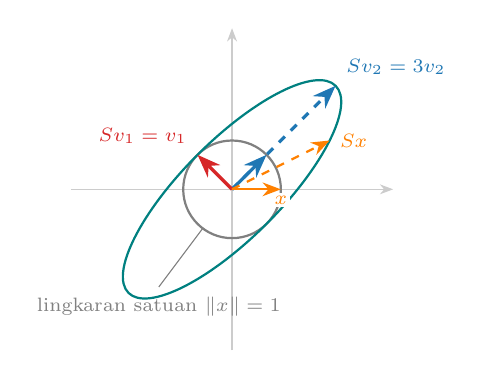
\begin{tikzpicture}[scale=0.62, >=Stealth]
  \draw[gray!40, ->] (-3.3,0) -- (3.3,0);
  \draw[gray!40, ->] (0,-3.3) -- (0,3.3);
  % lingkaran satuan
  \draw[thick, gray] (0,0) circle (1);
  % citra: elips S*x (sumbu 3 arah (1,1), sumbu 1 arah (-1,1))
  \draw[thick, teal, rotate=45] (0,0) ellipse (3 and 1);
  % vektor eigen
  \draw[->, very thick, kolom] (0,0) -- (0.707,0.707);
  \draw[->, very thick, kolom, dashed] (0,0) -- (2.121,2.121)
        node[above right, font=\scriptsize] {$Sv_2 = 3v_2$};
  \draw[->, very thick, baris] (0,0) -- (-0.707,0.707)
        node[above left, font=\scriptsize] {$Sv_1 = v_1$};
  % vektor biasa
  \draw[->, thick, orange] (0,0) -- (1,0) node[below=1pt, font=\scriptsize, fill=white, inner sep=1pt] {$x$};
  \draw[->, thick, orange, dashed] (0,0) -- (2,1)
        node[right, font=\scriptsize] {$Sx$};
  \draw[gray, thin] (-0.6,-0.8) -- (-1.5,-2.0)
        node[below, font=\scriptsize] {lingkaran satuan $\|x\|=1$};
\end{tikzpicture}
\column{0.44\textwidth}
\small
Setiap titik $x$ di \alert{lingkaran satuan} dipetakan ke $Sx$; hasilnya
\textcolor{teal}{elips}.
\begin{itemize}
  \item Vektor biasa ($x$) \textbf{berbelok} arahnya.
  \item Vektor eigen \textbf{tetap searah}; panjangnya dikali $\lambda$.
  \item Sumbu elips = arah vektor eigen, panjang semi-sumbu = $|\lambda|$.
  \item Luas elips $= |\det S|\cdot\pi = 3\pi$.
\end{itemize}
\end{columns}
\end{frame}

% ---------------------------------------------------------------------
\begin{frame}[fragile]{Membuat gambar lingkaran satuan di MATLAB}
\begin{columns}[T]
\column{0.58\textwidth}
\begin{lstlisting}[basicstyle=\ttfamily\footnotesize]
S = [2 1; 1 2];
t = linspace(0, 2*pi, 200);
X = [cos(t); sin(t)];     % lingkaran satuan
Y = S * X;                % citra: elips

[V, D] = eig(S);
plot(X(1,:), X(2,:), 'k'), hold on
plot(Y(1,:), Y(2,:), 'b')
quiver(0, 0, V(1,1), V(2,1), 0, 'r')
quiver(0, 0, V(1,2), V(2,2), 0, 'g')
axis equal, grid on, hold off
\end{lstlisting}
\column{0.38\textwidth}
\small
\begin{itemize}
  \item Setiap kolom \texttt{X} adalah satu titik di lingkaran.
  \item \texttt{S*X} mentransformasi semua titik sekaligus.
  \item \texttt{axis equal} wajib agar lingkaran tidak tampak lonjong.
\end{itemize}
\vspace{0.3em}
\scriptsize Demo interaktif klasik MATLAB untuk ide ini bernama
\texttt{eigshow}; di rilis baru mungkin tidak tersedia bawaan.
\end{columns}
\end{frame}

% ---------------------------------------------------------------------
\begin{frame}{Ringkasan operasi matriks}
\small
\renewcommand{\arraystretch}{1.25}
\centering
\begin{tabular}{l l l}
\toprule
Operasi & MATLAB & Catatan \\
\midrule
Penjumlahan / pengurangan & \texttt{P+Q}, \texttt{P-Q} & ukuran harus sama \\
Perkalian matriks & \texttt{A*B} & kolom $A$ = baris $B$; tidak komutatif \\
Perkalian skalar & \texttt{k*A} & tiap elemen dikali $k$ \\
Kronecker & \texttt{kron(A,B)} & blok $a_{ij}B$; ukuran $mp\times nq$ \\
Transpose & \texttt{A'}, \texttt{A.'} & \texttt{'} mengonjugasi bilangan kompleks \\
Determinan & \texttt{det(A)} & faktor skala luas; jangan untuk uji singular \\
Invers & \texttt{inv(A)}, \texttt{A\textbackslash b} & pakai \texttt{\textbackslash} untuk SPL \\
Nilai/vektor eigen & \texttt{[V,D] = eig(A)} & $Av=\lambda v$ \\
Diagonalisasi & \texttt{V*D/V} & $A = VDV^{-1}$ \\
\bottomrule
\end{tabular}
\end{frame}

\end{document}
